\lstdefinestyle{mystyle}{
    backgroundcolor=\color{myyellow},
    basicstyle=\ttfamily\small,
    breaklines=true,
    frame=single,
    language=XML
}

\chapter{State-of-the-Art Analysis} \label{ch:state-of-the-ArtAnalysis}
The following chapter constitutes an in-depth exploration of current technologies and methodologies within the automotive industry, with a specific focus on the complexity of vehicular software development. Firstly, the current automotive landscape will be examined, providing a detailed insight into challenges associated with software development in vehicles.

Subsequently, through meticulous analysis of scientific publications, technical reports, and practical implementations, the chapter delves into the radical transformation of the automotive sector facilitated by the concept of \gls{ac:sdv}. This technology, crucial for technological progress and vehicular safety, will be explored from various perspectives. Particularly, the synergy between cloud computing, software, and hardware will be investigated, highlighting solutions proposed by major industry players and analyzing their applications, benefits, and limitations.

The objective is to offer a comprehensive overview of current dynamics, emphasizing the pivotal role of \gls{ac:sdv} in the evolution of the automotive industry.

\section{Context}

In the past, the automotive industry advanced primarily through the development of technologies in mechanical engineering, focusing on perfecting combustion engines. Nowadays, the paradigm has radically changed due to multiple factors, including electrification, automation, shared mobility, and connected mobility.

Software technology development in the automotive field can be metaphorically compared to what has happened in smartphone development, as highlighted in the manifesto document regarding \textit{Bosch}'s \gls{ac:sdv} \cite{SDVBoschMobility}.

The ultimate goal is to achieve simple and user-friendly devices that fully meet the user's needs. Currently, many customers express dissatisfaction because their cars do not offer the same functionality and ease of use common in smartphones. Many ask the question about how is possible that their \$50,000 car can't perform the same tasks as their \$300 smartphone.

A key difference between the automotive and smartphone industries is the level of complexity, which brings with it a number of issues.

\subsection{difficulties}
It is possible to analyse in depth the problems of the current automotive software that is being developed via four main difficulties:

\begin{itemize}
    \item \textbf{Specialized Hardware:} Today's vehicles are still complex systems of systems. Each subsystem in a car, from brakes to transmission, is a complex entity, supplied by a different manufacturer and integrated with a unique software architecture. The level of complexity and the need for seamless interoperability between systems far exceeds that of today's smartphones.
    \item \textbf{Time:} The software production pipeline involves many development and testing steps with a not inconsiderable amount of time spent on each one. This is greatly increased by the presence of different components, so development time must be considered for each different unit of the system.
    \item \textbf{Cost:} The complexity of the software systems in vehicles entails very high costs, aggravated by the fact that the test phase is often carried out directly on the boards (for hardware requirements), which means a much longer production process, especially in the event of errors.
    
    \begin{table}[h]
        \begin{tikzpicture}
            \begin{axis}[
                width=13cm,
                height=12cm,
                xlabel={Life cycle phases}, ylabel={Relative cost of error fixing},
                xtick={1.6, 2.1, 3.3, 3.9, 4.9},
                xticklabel style={rotate=0, anchor=east, yshift=-12pt},
                xticklabels={ \shortstack{Requirements}, \shortstack{Design}, \shortstack{Implementation}, \shortstack{Testing}, \shortstack{Distribution  \& \\ Maintenance}},
                ymin=0,
                ymax=100,
                ytick={0, 50, 100}
            ]
            \addplot+[mark=none, smooth, domain=1:5, samples=100] {10*exp(0.5*x)};
            \legend{Cost of fixing in time}
            \end{axis}
            \end{tikzpicture}
        \caption{Cost of fixing errors increases in later phases of the life cycle \cite{CostsOfSoftwareDeveloping}}
        \label{tab:CostsOfSoftwareDeveloping}
    \end{table}

    \item \textbf{Human Safety Security:} Automotive embedded software must meet stringent reliability and security requirements, while delivering performance and a reasonable memory footprint. To develop automotive embedded software, you need the right tools that meet safety and security standards to evaluate, prototype and test your software.
\end{itemize}

At this point, Several valuable lessons can be learned from studying the barriers that apply to the vehicle life cycle. Historically, the vehicle lifecycle has been characterised by the simultaneous production and deployment of tightly integrated hardware and software. Once the vehicle was in the hands of the consumer, its characteristics remained largely unchanged until the end of its life. However, the \gls{ac:sdv} paradigm introduces the possibility of decoupling hardware and software release dates, a prerequisite for adopting a digital-first approach. This approach brings the design and virtual validation of the digital vehicle experience to the forefront of the lifecycle.
It also requires the application of the digital-first concept, which means that new ideas for the vehicle experience are first explored in virtual environments to ensure early user feedback, long before any custom hardware needs to be developed or a physical test vehicle is available. Digital first is the application of design thinking and lean startup principles, originally rooted in internet culture, to the tangible realm of automotive development.

%“Automakers and their suppliers need to continuously review and improve the testing approach in design and development, as well as look for new tools that automate and increase test coverage of their products,” Giallorenzo explained. “Cloud emulation is a major innovation that is coming to the industry to facilitate development and testing. Historically, testing of embedded software solutions has been hindered by the lack of chipsets and hardware, which is required to properly test complete hardware-plus-software solutions. This was particularly painful during the recent COVID-induced supply chain crunch."

\section{Introduction to Software Defined Vehicle}
The \gls{ac:sdv} represents the new frontier of automotive manufacturing and is poised to completely change the paradigm of automotive production. 

Let's try to imagine to bringing a feature update to one of today's vehicles. It will most likely take anywhere from one to seven years from the idea to when that feature is actually perceptible in the production vehicle; this takes so long because the vehicles produced up to this point have not been designed with frequent updates in mind \cite{SDVBosch}.
Traditionally focused on physical functionality, the automotive industry has evolved from early electronic features such as airbags, vehicle stabilisation and braking systems to modern driver assistance and even automated driving. 
The current shift towards a digital experience is possible thanks to vehicle design that includes software integration as a fundamental part. Software should no longer be seen as an accessory to the vehicle, but as an integral part of the vehicle itself.

The simultaneous efforts of major automotive companies such as \textit{Bosch}, \textit{Renault} and \textit{Stellantis}, in collaboration with leading computer developers such as \textit{Arm}, \textit{BlackBerry} and \textit{\gls{ac:aws}}, have given rise to the \gls{ac:sdv} concept, which they define as "any vehicle that manages its own operations, adds functionality and enables new features primarily or entirely through software" \cite{blackberrySDV}.

The \gls{ac:sdv} solution is nowadays being considered by several companies as the manifesto of a new era of vehicle development. An example is given by the \textit{Renault Group}, which in an overview of its products describes: "Today, it is already possible to make remote updates of some vehicles via the \gls{ac:fota} system. This keeps the vehicle safe by making it easier and faster to improve the on-board system and apply patches. Tomorrow, the \gls{ac:sdv}'s flexible and scalable architecture will enable the faster development and integration of new features throughout the vehicle lifecycle, directly into the cloud, that is, in secure online servers accessible from anywhere and anytime" \cite{SDVRenault}. 

It is evident that \gls{ac:sdv}s represent the future of the automotive industry, promising an enriched and sustainable user experience as vehicle technologies evolve. This section further clarifies the current state of the industry, highlighting the key enablers that are allowing the development of the \gls{ac:sdv} paradigm and the benefits of this innovation.

\subsection{Enablers}

There are mainly four fundamental technologies that contribute to the realisation of the \gls{ac:sdv}: standardized hardware, cloud, \gls{ac:ota} updates via \gls{ac:ota} servers, and \gls{ac:mqtt} communication. All these enablers are developed by leading companies in the computing industry. In this section, each technology will be analysed with reference to concrete examples from the current market.

\begin{itemize}
    \item[] \textbf{Standardized hardware} 
    
    One of the most important aspects of \gls{ac:sdv} is the separation of software from hardware. To achieve this, it is essential to move away from the approach of using dedicated hardware for each vehicle component system, and instead favour an approach based on general purpose processors that are as centralised as possible. This transition not only promotes ease of software development and scalability, but also offers the opportunity to create parity between the virtual development and test environment and the real execution environment.
    
    Several players in the semiconductor industry have stepped up to the challenge of realising this vision, including \textit{Arm}. Through the development of energy-efficient processors, \textit{Arm} is present in every part of the vehicle, from high-performance systems in \gls{ac:adas}, \gls{ac:ad}, \gls{ac:ivi} and digital cockpits, to gateway, body and microcontroller endpoints \cite{ArmAutomotive}. The aim is to create Arm-based \gls{ac:mcu}s that enable implementation of a common architecture, scalability between applications to meet processing requirements, software reuse and reduced development costs.
    
    Another major player is \textit{Qualcomm}, which is being adopted by the \textit{Renault Group} through its \textit{Snapdragon Digital Chassis} vehicle architecture, a set of cloud-connected platforms for telematics and connectivity, digital cockpits, assistance and driver autonomy.

    \item[] \textbf{Cloud} 
    
    Using a cloud platform that offers scalable and secure solutions for real-time application updates, increased connectivity and efficient data management is essential for \gls{ac:sdv}. 

    Well-known companies such as \textit{\gls{ac:aws}} and \textit{Google Cloud} are already present in the automotive industry as partners of partner of many automotive companies. The \gls{ac:aws} services and technologies will be in depth described in the futher chapters.
 
    \item[] \textbf{Over-The-Air updates}
    
    An \gls{ac:ota} update is the remote and wireless transfer of applications, services, firmware and configurations from a server to a target device. This process takes place over an available network, preferably the Internet. The main purposes of \gls{ac:ota} are to remotely update software or firmware, provide power-safe procedures to ensure that the device will boot even if power is lost during the update process, maintain a robust implementation, ensure data protection and reduce overall maintenance costs \cite{Open-sourceSWUpdate}.

    In the context of the thesis, it is crucial to acknowledge that the implementation of \gls{ac:ota} updates may increase the vulnerability of automotive systems to hacking and other cyber attacks. These vulnerabilities could potentially be exploited by hackers to gain unauthorised access to private information, take remote control of the vehicle or even cause it to malfunction. Another significant issue is the leakage of information about updates and their sources. This can enable malicious actors to introduce viruses and malware, further exacerbating the security risks associated with \gls{ac:ota} updates \cite{EnhancedMulti-LevelSecureUpdate}. 
    
    To perform an \gls{ac:ota} update, both a client on the vehicle, responsible for waiting and checking for incoming updates, and a server, facilitating the availability of the update broadcast to all connected devices, are essential. In this context, Autosar can be considered, as it represents a standard and open source architecture for intelligent mobility \cite{AutosarAbout}, which includes a dedicated platform for client and server management of \gls{ac:ota} updates. Another notable example is Hawkbit, which serves as a backend framework for deploying software updates to edge devices and is being developed by the Eclipse Foundation; this tool will be discussed in more detail in later chapters as it will be used to create a proof of concept. The final tool of note is AWS Greengrass, an edge agent manager for managing software updates in edge \gls{ac:iot} devices, provided by AWS; this tool will also be discussed in later chapters as an alternative solution to the client manager.
    
    \item[] \textbf{MQTT communication}
    
    The \gls{ac:mqtt} is a standardized protocol, specified by \textit{ISO/IEC 20922:2016} and developed by the \textit{Oaesis} organization. It enables the exchange of \textit{\gls{ac:am}} over a network connection, providing an ordered, lossless stream of bytes from the \textit{Client} to \textit{Server} and \textit{Server} to \textit{Client} without the need to support of a specific transport protocol.

    In an \gls{ac:mqtt} transport, an \gls{ac:am} carries payload data, a \gls{ac:qos}, a collection of \textit{Properties}, and a \textit{\gls{ac:tn}}. \textit{Clients}, which can be programs or devices, perform various actions such as opening and closing network connections, publishing \textit{\gls{ac:am}}, subscribing to requested \textit{\gls{ac:am}}, and managing subscriptions \cite{MQTTVersion5.0}.

    On the \textit{Server} side, it acts as an intermediary between publishing and subscribing \textit{Clients}. The \textit{Server} accepts network connections, processes \textit{Subscribe} and \textit{Unsubscribe} requests, and forwards \textit{\gls{ac:am}} matching \textit{Client Subscriptions}. The \textit{Server}, also known as the \textit{Broker}, essentially coordinates messages among various \textit{Clients}. Its responsibilities extend to authorizing and authenticating \textit{\gls{ac:mqtt} Clients}, transmitting messages to other systems for further analysis, and managing tasks such as handling missed messages and \textit{Client} sessions \cite{MQTTAWS}.

    Sessions, representing stateful interactions between Clients and Servers, can last for the duration of a Network Connection or span multiple consecutive connections.
     \begin{figure}[h]  % 'h' significa che la figura viene posizionata qui
        \centering
        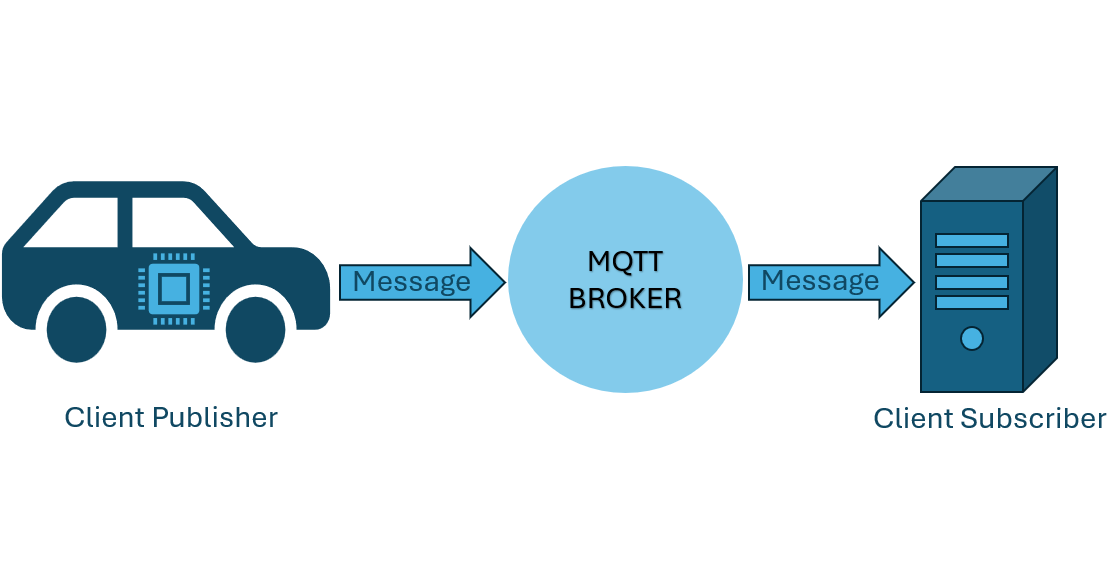
\includegraphics[width=0.8\textwidth]{images/MQTTProtocol.png}  % Sostituisci 'nome_immagine' con il nome del tuo file immagine e l'estensione
        \caption{A simple representation of communication using the \gls{ac:mqtt} protocol}
        \label{fig:MQTTProtocol}
    \end{figure}

    The \gls{ac:mqtt} protocol can be used in \gls{ac:sdv}, both for sending data produced by the vehicle to the cloud servers and for sending updates from the servers to the vehicle. This is because the \gls{ac:mqtt} protocol allows asynchronous and misaligned communication even in the presence of poor connectivity, a situation that cannot be underestimated in the automotive field.
\end{itemize}

The collaborative efforts of this technologies contribute to advancement of \gls{ac:sdv} for makeing vehicles not only defined by their physical attributes but also as dynamic entities that can be continuously updated through software.

\subsection{Benefits}
The \gls{ac:sdv}, as introduced in the previous chapters, brings several benefits to both automotive companies and the end-user experience.  These innovations are made possible by the fact that the vehicle becomes a device that can be constantly monitored and updated in real time via the cloud throughout its entire lifecycle. Let us now look at the key benefits.

From the point of view of this project, the main innovation brought by this technology is the security of the device software. Since, as mentioned above \cite{ISO26262}, vehicles are considered as safety elements critical to human life, the safety benefits can be analysed from two perspectives:
\begin{itemize}
    \item \textbf{Human Safety Critical Security:} The ability of \gls{ac:sdv} to receive real-time data from the vehicle allows in-depth monitoring of all its components. Taking the influence of tyres as an example, it has been found that most road accidents are caused by tyre wear and lack of regular maintenance. It is therefore necessary to assess the health of tyres through continuous monitoring of physical parameters such as tyre thickness, temperature and pressure, as well as regular maintenance. This helps to eliminate or minimise the possibility of tyre bursts and subsequent accidents. It also improves the safety of people and vehicles \cite{PredictDefectsOfTiresInHeavyVehicle}. These factors can be monitored either manually or automatically: manual predictive maintenance requires human intervention and can lead to some errors; automatic predictive maintenance using artificial intelligence can be more efficient \cite{AirPressureSystemFailurePrediction}. \textit{Renault} defines this work as "predictive maintenance" \cite{SDVRenault}, stressing the importance of collecting and analysing data in a centralised system to anticipate and prevent potential failures, ensure the safety of people, reduce maintenance costs and improve the performance of the vehicle.
    \item \textbf{Intrinsic Software Security:} In the presence of bugs and vulnerabilities in the vehicle's software, \gls{ac:sdv} makes it possible to intervene promptly to resolve each problem and reduce the window of exposure.
    \begin{table}[h]  % 'h' significa che la figura viene posizionata qui
        \centering
        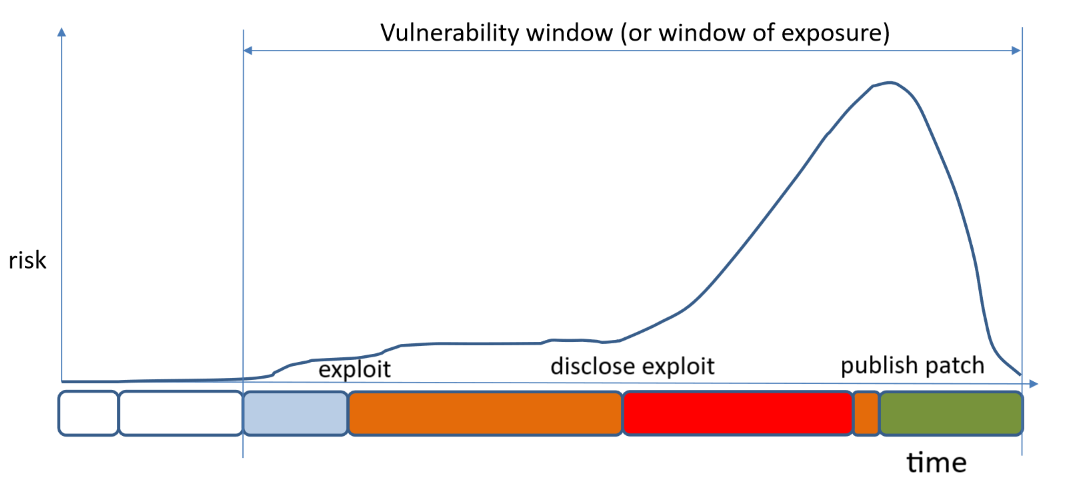
\includegraphics[width=0.8\textwidth]{images/window_of_exposure.png}  % Sostituisci 'nome_immagine' con il nome del tuo file immagine e l'estensione
        \caption{Risks and time relationship in the various phases of a vulnerability lifecycle}
        \label{tab:WindowOfExposure}
    \end{table}

    A crucial aspect of vehicle software security is the robustness of the algorithms, especially in the context of autonomous driving. In this context, a predictive algorithm responsible for vehicle safety decisions can be continuously improved and optimised. The \gls{ac:sdv} also introduces the concept of the \textit{Digital Twin}, that is a platform that virtually replicates the functionality and behaviour of the vehicle in a computing environment. Thanks to this technology, predictive algorithms used in autonomous driving can be effectively tested on the cloud platform and, when ready, integrated directly into the vehicle.
\end{itemize}

From a user experience point of view, two other significant benefits can be identified: an increase in the value of the vehicle, which can be continuously upgraded over time, and the ability to enable additional vehicle functions via software. For example, the user can decide to activate a feature for a certain period of time and then deactivate it (paying only for the time it is used), or activate a new feature that was not available at the time of purchase. In essence, the vehicle becomes a dynamic platform that is constantly evolving and fully customisable through the software.

For automotive companies, the benefits mentioned so far can bring direct advantages to the entire industry. In support of this, \textit{Stellantis} reports that: "the team in Poland will contribute to the global software creation network that is key to Stellantis' work in creating \gls{ac:sdv} that offer customer-focused features throughout the vehicle's life span, including updates and features that will be added years after the vehicle is manufactured. Creating an infrastructure inside our vehicles that easily and seamlessly adapts to meet driver expectations is a key element of Stellantis' global drive to deliver cutting edge mobility. Stellantis' software-driven strategy deploys next-generation tech platforms, building on existing connected vehicle capabilities to transform how customers interact with their vehicles and to generate €20 billion in incremental annual revenues by 2030" \cite{StellantisSDV}.

In addition, the \gls{ac:sdv} paradigm brings an advantage from a software production pipeline perspective. In today's software production scenario, there can be two development mechanisms:
\begin{itemize}
    \item A more traditional mode in which software is created directly on the system, hence on the processor itself. This is undoubtedly the most inconvenient solution, as it would require unnecessary overuse of processors, wasting resources, money and time.
    \item Alternatively, developers rely on cumbersome operating system emulation tools on the host machine and the cross-compilation process, which uses a dedicated compiler to produce executable code for the target system. Once the code is on the development system, a final integration and validation test can be performed, but scalability is limited to the number of physical hardware platforms. 
\end{itemize}

Typical workflows for the development, integration and validation of embedded systems are as follows:
\begin{figure}[h]  % 'h' significa che la figura viene posizionata qui
    \centering
    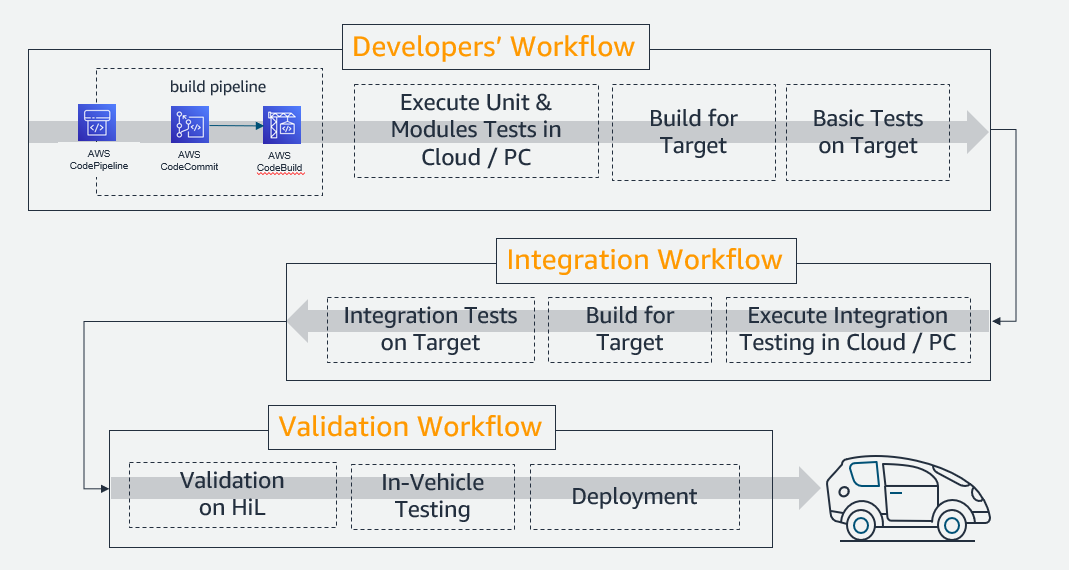
\includegraphics[width=0.7\textwidth]{images/today_developer_workflow.png}  % Sostituisci 'nome_immagine' con il nome del tuo file immagine e l'estensione
    \caption{today development, integration, and validation workflows for embedded systems \cite{DevelopersWorkflow}.}
    \label{fig:TodayDeveloperWorkflow}
\end{figure}

By using the \gls{ac:sdv}, such as operating systems that rely on general porpouse architectures to provide parity between cloud and edge systems, it is possible to reduce the embedded developer's workflow to remove many of the steps that are now no longer required, as shown in the diagram below \ref{fig:FutureDevelopersWorkflow}. More specifically, the development and integration workflow eliminates the build and test phases. Instead, a validation function is added to verify the product in a cloud environment, where the digital twin concept can be used directly. All tests can be conducted in a virtual cloud environment where a digital copy of the actual vehicle is available for distributing the product software or related updates. This reduces software production times, costs, and waste of physical resources.
\begin{figure}[h]  % 'h' significa che la figura viene posizionata qui
    \centering
    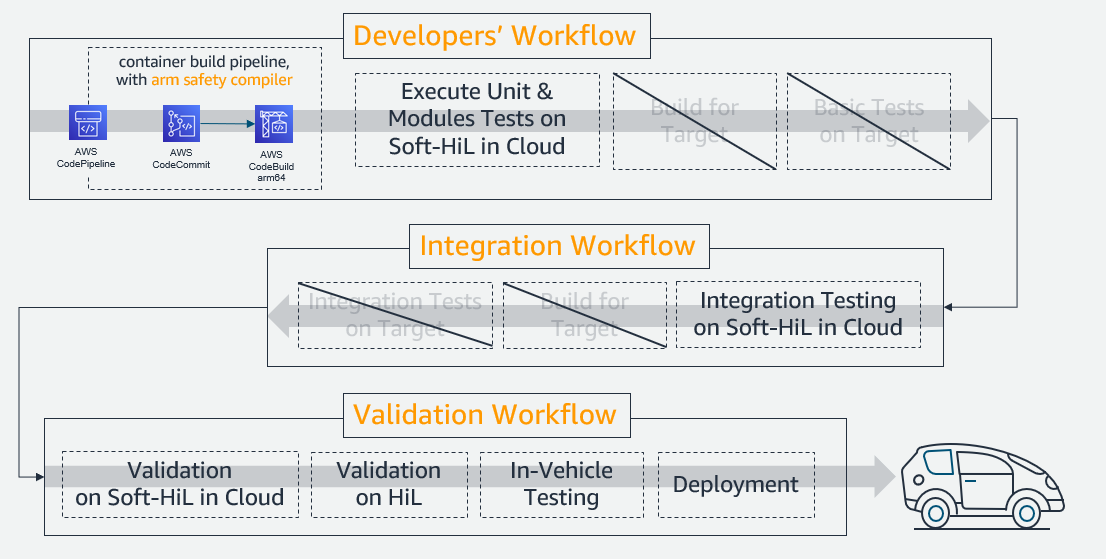
\includegraphics[width=0.7\textwidth]{images/future_developers_workflow.png}  % Sostituisci 'nome_immagine' con il nome del tuo file immagine e l'estensione
    \caption{future development, integration, and validation workflows for embedded systems \cite{DevelopersWorkflow}.}
    \label{fig:FutureDevelopersWorkflow}
\end{figure}

\subsection{initiatives: SOAFEE}
In 2021 \textit{Arm}, \textit{\gls{ac:aws}}, and other founding members announced the \textit{\gls{ac:soafee} Special Interest Group}, which brings together automakers, semiconductor, and cloud technology leaders to define a new open-standards based architecture to implement the lowest levels of a software-defined vehicle stack \cite{DevelopersWorkflow}.

\gls{ac:soafee} is created to achive \gls{ac:sdv} objective, and for doing that four-pillar principle are used \cite{SoafeeProject}:
\begin{enumerate}
    \item \textbf{Standards:} standardization ensures interoperability and compatibility among various software components, fostering a cohesive ecosystem for \gls{ac:sdv}s.
    \item \textbf{New software architecture and methodologies:} this involves transitioning from traditional monolithic architectures to more modular and scalable designs; the incorporation of agile development practices and \textit{DevOps} methodologies ensures efficient and continuous software evolution.
    \item \textbf{Industry collaboration:} Fostering partnerships, knowledge sharing and collaboration among key stakeholders, including automakers, technology companies and regulators, is essential.
    \item \textbf{Vehicle simulation:} simulated environments allow in-depth testing and refinement of software functionality to ensure optimal performance and security under a variety of conditions.
\end{enumerate}
\gls{ac:soafee} aims to adopt and enhance current standards used in today's cloud-native world to help manage the software and hardware complexity of the automotive \gls{ac:sdv} architecture.

The core principles of safety, security, and real time are inherent in each pillar. It is fully expected that the \gls{ac:soafee} architecture will support use-cases that execute safety-critical services alongside non-safety-critical ones. It is fully expected that the \gls{ac:soafee} architecture will support use cases that execute safety-critical services alongside non-safety-critical services. As it is not reasonable to develop the whole platform according to one safety standard, the strategy is to develop only safety-critical elements according to \textit{\gls{ac:iso} 26262} and to isolate them from the non-safety-critical elements in order to ensure spatial, temporal and communication isolation. All implementations pass security checks and follow a set of best practices \cite{SoafeeArchitectureOverview}.

The \gls{ac:soafee} paradigm is based on a very sophisticated architecture becouse it should work in the same way in the vehicle and in the cloud and follow cloud native technologies while considering the automotive specific needs for safety and limited resource footprints \cite{SoafeeArchitecture}.
\begin{figure}[h]  % 'h' significa che la figura viene posizionata qui
    \centering
    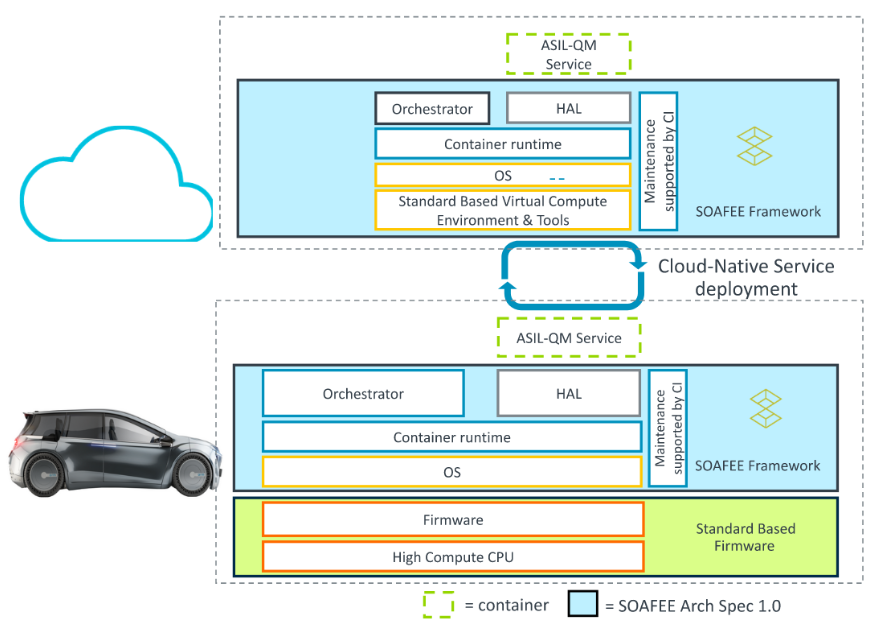
\includegraphics[width=0.7\textwidth]{images/SOAFEE_architecture.png}  % Sostituisci 'nome_immagine' con il nome del tuo file immagine e l'estensione
    \caption{\gls{ac:soafee} Architecture v1.0 \cite{SoafeeArchitecture}}
    \label{fig:SoafeeArchitecture}
\end{figure}